\bsection{Skill List}
\subsection*{Combat Skills}
\textbf{Ambidextrous} the warrior is adept at two weapon fighting and may ignore the dual wielding penalty. \\
\textbf{Strike to Injure} Add +1 to all injury rolls caused
by the model in hand-to-hand combat. \\
\textbf{Combat Master} If he fights against more than one
enemy at a time, he gains an extra Attack in each
hand-to-hand combat phase as long as he is fighting
two or more enemy models. In addition, the warrior
is immune to ‘All Alone’ tests. \\
\textbf{Weapons Training} The warrior may use any hand-
to-hand combat weapon he comes across, not just
those in his equipment options.\\
\textbf{Web of Steel} The model gains +1 to all his rolls on
Critical Hit tables in hand-to-hand combat. \\
\textbf{Expert Swordsman} The warrior may re-roll all
missed attacks if he is using a sword in the hand-to-
hand phase of the turn that he charges. Note that this
only applies when they are armed with normal
swords or weeping blades, and not with double-
handed swords or any other weapons. \\
\textbf{Step Aside} Each time he suffers a wound in close
combat he may make an additional saving throw of
5+. This save is never modified and is taken after all
other armour saves.
\subsection*{Shooting Skills}
\textbf{Eagle Eyes} The warrior adds +6” to the range of any missile weapon he is using. \\
\textbf{Hunter} The warrior may fire each turn with a handgun or Hochland long rifle. \\
\textbf{Knife-Fighter} The warrior can throw a maximum of three of these missiles in his shooting phase and may divide his shots between targets. Cannot be combined with Quick Shot. \\
\textbf{Nimble} The warrior may move and fire with weapons that are normally only used if the firer has not moved. Note that this skill cannot be combined with the Quick Shot skill. \\
\textbf{Pistolier} If he is equipped with a brace of pistols of any type (including crossbow pistols), he may fire twice in the Shooting phase (though note that normal reloading rules apply). If he has a single pistol then he may fire it in the same turn it was reloaded. \\
\textbf{Quick Shot} The warrior may shoot twice per turn with a bow or crossbow (but not a crossbow pistol). \\
\textbf{Trick Shooter} The warrior ignores all modifiers for cover when using missile weapons. \\
\textbf{Weapons Expert} The warrior may use any missile weapon he comes across, not just the weapons available from his list.
\subsection*{Academic Skills}
\textbf{Arcane Lore} Any warrior with this skill may learn Lesser Magic if he owns a Tome of Magic. Not available to Sisters or Witch Hunters. \\
\textbf{Battle Tongue} This skill may only be chosen by a leader. This increases the range of his Leader ability by 6”. Not available to Undead leaders. \\
\textbf{Haggle} The warrior may deduct 2D6 gold crowns from the price of any single item (to a minimum of 1gc) once per post battle sequence. \\
\textbf{Hunch} only for leader. Place up to 3 men capable of earning experience into ruined building (at least 12” away from enemy) (see ”Ye Old Curiosity Shoppe”). \\
\textbf{Magical Aptitude} cast 2 spells in one turn by making a T test, roll ijury table if failed (see ”Ye Old Curiosity Shoppe”). \\
\textbf{Mind Focus} reroll one dice roll in casting spells (see ”Ye Old Curiosity Shoppe”). \\
\textbf{Scribe} once per battle +2 to spell roll (see ”Ye Old Curiosity Shoppe”). \\
\textbf{Sorcery} A warrior with this skill gains +1 to his rolls to see whether he can cast spells successfully or not. Not available to Sisters or Witch Hunters. \\
\textbf{Streetwise} The warrior may add +2 to the roll that determines his chances of finding such items. \\
\textbf{Tactician} only for leader. May reposition his warriors after setup, and move borders to 12” (see ”Ye Old Curiosity Shoppe”). \\
\textbf{Warrior Wizard} This skill may only be taken by spellcasters. The mental powers of the wizard allow him to wear armour and cast spells. \\
\textbf{Wyrdstone Hunter} If a Hero with this skill is searching the ruins in the exploration phase you may re-roll one dice when rolling on the Exploration chart. The second result stands.
\subsection*{Strength Skills}
\textbf{Mighty Blow} The warrior knows how to use his strength to maximum effect and has a +1 Strength bonus in close combat. \\ 
\textbf{Pit Fighter} The warrior is an expert at fighting in confined areas and adds +1 to his WS and +1 to his Attacks if he is fighting inside buildings or ruins. \\ 
\textbf{Resilient} Deduct -1 Strength from all hits against him in close combat. This does not affect armour save modifiers. \\ 
\textbf{Fearsome} Such is the reputation and physique of the model that he causes fear in opposing models. \\ 
\textbf{Strongman} The warrior may use a double-handed weapon without the usual penalty of always striking last. Work out order of battle as you would with other weapons. \\ 
\textbf{Unstoppable Charge} The warrior adds +1 to his Weapon Skill when charging.
\subsection*{Speed Skills}
\textbf{Leap} The warrior may leap D6” in the movement phase in addition to his normal movement. He may move and leap, run and leap, or charge and leap, but he can only leap once per turn. A leaping warrior may jump over opposing man-sized models, including enemies, and obstacles 1” high, without penalty. The leap may also be used to leap over gaps, but in this case you must commit the warrior to making the leap before rolling the dice to see how far he jumps. If he fails to make it all the way across, he falls through the gap. \\
\textbf{Sprint} The warrior may triple his Movement rate when he runs or charges, rather than doubling it as normal. \\
\textbf{Acrobat} The warrior may fall or jump from a height of up to 12” without taking any damage if he passes a single Initiative test, and can re-roll failed Diving Charge rolls. He can still only make a diving charge from a height of up to 6”. \\
\textbf{Lightning Reflexes} The order of attack between the warrior with this skill and his opponent(s) when being charged is determined by comparing Initiative value. \\
\textbf{Jump Up} The warrior may ignore knocked down results when rolling for injuries, unless he is knocked down because of a successful save from wearing a helmet or because he has the No Pain special rule. \\
\textbf{Dodge} The warrior can avoid any hits from a missile weapon on a D6 roll of 5+. Note that this roll is taken against missiles as soon as a hit is scored to see whether the warrior dodges it or not, before rolling to wound, and before any effects from other skills or equipment (such as lucky charms). \\
\textbf{Scale Sheer Surfaces} The warrior can climb up or down a height equal to twice his normal Movement, and does not need to make Initiative tests when doing so.
\bsection{Special Skills}

Listed in band's description.

If Hired Sword gains enough experience for
an advance, roll on the Heroes Advancement table (as
opposed to Henchmen) to determine which advance
he gains. Skills available to the Hired Swords are
listed under their entries. Some hirelings can learn special skills from their description.

\vspace*{-1cm}\hspace*{2.1cm}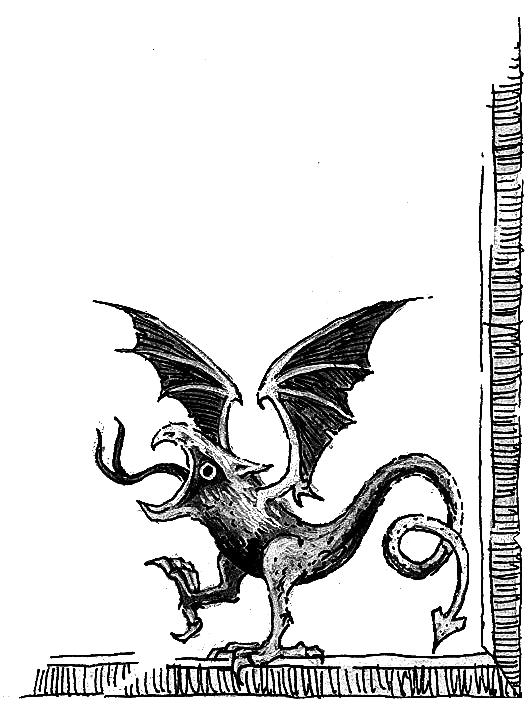
\includegraphics[height=5.3cm]{corner}